\documentclass[journal]{IEEEtran}


\usepackage{graphicx}
\usepackage[caption=false,font=footnotesize]{subfig}
\usepackage{cite}
\usepackage{amsmath,amsthm,amssymb}
\usepackage{rotating}

\usepackage{pbox}
%\usepackage{geometry}
%\usepackage[margin=1in]{geometry}
\usepackage{array}
\usepackage{multirow}
\usepackage{xcolor}
\usepackage{listings}
\usepackage{booktabs}
\usepackage{mathtools}

\usepackage{algorithm}
\usepackage{algpseudocode}
%\usepackage{algorithmic}
\usepackage{comment}
\usepackage{scalerel}


\usepackage{tikz}
\usetikzlibrary{arrows.meta, positioning, shapes.multipart, shadows, decorations.pathreplacing}

\usepackage{hyperref}
\hypersetup{hidelinks}

\hyphenation{op-tical net-works semi-conduc-tor IEEE-Xplore}

% Results directories (relative to the paper/ folder)
\newcommand{\cicresults}{../results/darknet_ci/seed_1}
\newcommand{\cicaggresults}{../results/darknet_ci/aggregate}
\newcommand{\vpnresults}{../results/iscx_full}

\begin{document}

\title{Durability Deception: Concept Drift in Encrypted Traffic Classifiers and a Continual Learning Defense}

\author{Benjamin Appiah, Daniel Commey, Isaac Osei, Gabriel Assamah, Alimatu Saadia Yussiff, Ebenezer Owusu}


\maketitle

\begin{abstract}
State-of-the-art encrypted traffic classification models often achieve near-perfect accuracy under static evaluation, yet suffer silent performance collapse after deployment due to temporal concept drift—a failure mode we term the \textit{durability deception}. We present a systematic temporal analysis of this phenomenon on the CICDarknet2020 dataset, revealing a \textbf{91\%} relative macro-F1 drop from the first to the final window under chronological evaluation. A static XGBoost classifier drops to \textbf{8.8\%} macro F1 in the final window and attains only \textbf{29.7\%} average F1 across the full horizon. To address this failure, we propose \textsc{LightGuard}, a continual learning framework that \emph{explicitly enforces model durability under drift} by coupling drift-aware adaptation with stability-preserving rehearsal. Rather than treating adaptation as ad hoc retraining, \textsc{LightGuard} operationalizes a principled stability–plasticity trade-off, selectively updating model parameters when distributional shifts are detected. Across long-horizon evaluations (mean over 3 seeds), \textsc{LightGuard} sustains \textbf{97.3\%} average macro F1 with minimal overhead, substantially outperforming both static models and replay-style proxy baselines (\textbf{72.9\%}). Our results establish durability as a first-class evaluation dimension for encrypted traffic classification and provide a practical yet principled pathway toward sustainable drift-aware encrypted traffic monitoring.
\end{abstract}


\begin{IEEEkeywords}
Concept Drift, Continual Learning, Encrypted Traffic Classification, Darknet Traffic, Model Durability.
\end{IEEEkeywords}


\section{Introduction}
\label{intro}
The growing prevalence of encrypted network traffic presents a fundamental challenge for modern network security systems. While encryption is indispensable for protecting user privacy, it simultaneously obscures payload content and renders traditional deep packet inspection ineffective. As a result, security teams increasingly rely on encrypted-traffic classification based on flow statistics to regain network visibility, for example distinguishing Tor- and VPN-routed traffic from other encrypted flows \cite{mdpi2022deep,Aceto_8640262}. To address this challenge, the research community has widely adopted machine learning (ML) techniques that operate on statistical flow features, achieving impressive performance under controlled evaluation settings \cite{SHARMA2025110984,sarhan2020standard,yang2021cade}.

Despite these successes, a critical gap persists between laboratory evaluations and real-world deployment. The majority of existing studies implicitly assume that network traffic distributions remain stationary over time, relying on random train–test splits of static datasets. Such evaluation protocols fail to capture the temporal evolution inherent to operational networks, where traffic characteristics continually shift due to software updates, protocol changes, evolving user behavior, and adaptive adversaries. This phenomenon, commonly referred to as \emph{concept drift} \cite{jiang2025adaptiveids,Uccello0_13,gehani2024safeguarding}, poses a severe threat to the longevity and reliability of ML-based encrypted-traffic monitoring systems.

In practice, models that initially exhibit near-perfect accuracy may experience substantial performance degradation months after deployment—often without explicit warning. We refer to this failure mode as the \emph{durability deception}: a misleading sense of security created by strong initial performance that masks silent degradation over time \cite{MALEKGHAINI2023109648,yang2021cade,webb2016characterizing}. While concept drift has been acknowledged in both machine learning and security literature, its long-term impact on encrypted traffic classification remains insufficiently quantified \cite{kumar2024adaptive}. Prior work has predominantly focused on optimizing static accuracy, offering limited insight into how quickly or severely deployed classifiers deteriorate when exposed to evolving traffic distributions \cite{singh2023comparative,MALEKGHAINI2023109648}. Consequently, a fundamental operational question remains unanswered: \emph{How durable are state-of-the-art encrypted traffic classifiers once deployed in dynamic network environments?} To address this gap, we make two primary contributions:
\begin{enumerate}
    \item We introduce a time-informed evaluation framework for encrypted traffic classification that explicitly accounts for temporal distribution shift. Using the CICDarknet2020 dataset as a primary testbed, we reframe static benchmarks into a chronological evaluation protocol and demonstrate that concept drift induces severe performance degradation in state-of-the-art models. This analysis establishes a quantitative benchmark for the \emph{durability deception}, revealing that celebrated accuracy scores can collapse when models are evaluated on evolved traffic distributions.
    
    \item We propose \emph{LightGuard}, a continual learning framework designed to preserve classification durability under non-stationary conditions. Rather than treating adaptation as ad hoc retraining, LightGuard operationalizes a principled stability–plasticity trade-off: it selectively initiates model updates only when drift is detected, while enforcing stability through rehearsal mechanisms that retain historically relevant knowledge. The update rule is model-agnostic in principle; in this paper we instantiate and evaluate it with tree-based ensembles (XGBoost).
\end{enumerate}
Our experimental results confirm the pronounced impact of concept drift on encrypted traffic classification using the CICDarknet2020 dataset \cite{habibi2022}, and demonstrate that LightGuard sustains high detection accuracy with minimal computational overhead. Additional validation on the ISCX-VPN dataset \cite{drapper2016} further supports the generalizability of our findings. By shifting the evaluation focus from one-time accuracy to long-term resilience, this work advances a more realistic foundation for deploying dependable ML-based security systems in operational environments.



\section{Related Work}
\label{sec:related_work}

\subsection{Static Classification of Encrypted Traffic}  
The majority of studies investigate methods which attain maximum precision when assessing unchanging encrypted traffic datasets. VPN and TLS classification benefits from the strong performance of ensemble methods which include Random Forest and stacking ensembles according to research conducted by \cite{eij2022vpn}. Later work employed deep learning architectures: CNNs for flow features or image-like packet blocks \cite{kumar2024adaptive,appiah2022fusion} and hybrid CNN/RNNs for spatial-temporal patterns \cite{mdpi2022deep}. While these improve accuracy, evaluations remain static, ignoring temporal dynamics in live networks.

\subsection{Adversarial Robustness in Traffic Classification} 
Another research avenue studies adversarial attacks on traffic classifiers. Crafted traffic features can deceive classifiers because they create conditions that replicate how attackers would try to stay undetected \cite{adeke2023securing,appiah2022fusion,sadeghzadeh2020adversarial}. Universal perturbations affect deep models which operate across multiple datasets \cite{ding2024towards}. Adversarial training alongside feature augmentation and randomness serves as main defense mechanisms against adversarial attacks \cite{adeke2023securing}. The system handles \emph{active} threats while it omits detection of passive traffic changes which result in natural performance deterioration.

 
\subsection{Sustainable and Adaptive Detection in Network Security}
Sustainability of ML-based security monitoring under drift has been studied in the broader intrusion detection and streaming learning literature. General adaptive approaches include:
Streaming anomaly detection systems (e.g., \cite{liu2021real}) apply online learning to flag deviations in real time, but typically rely on coarse volume-based signals rather than fine-grained encrypted traffic semantics. Adaptive intrusion detection explores mechanisms such as incremental clustering \cite{jiang2025adaptiveids,wang2022adaptive} and ensemble adjustment \cite{zhang2023dynamic} to track evolving behavior; however, many approaches depend on feature engineering tailored to unencrypted payloads or known attack signatures. Continual learning frameworks such as GEM \cite{lopez2017gradient} and EWC \cite{kirkpatrick2017ewc} are well-studied in general classification, yet their suitability for encrypted traffic—high-dimensional tabular features under strict privacy constraints—remains underexplored \cite{li2025continual}. In our experiments, we implement replay-style proxy baselines that capture the rehearsal intuition of these methods while remaining compatible with tree ensembles (XGBoost). While newer CL variants (e.g., DER++ \cite{buzzega2020}, GCR \cite{9880055}, ADAM-ER \cite{Li_2024}, CLIMB \cite{khosla2021}) are promising, their robustness to systematic temporal drift in encrypted traffic has not been validated.
In encrypted traffic classification, systematic temporal evaluation and dedicated continual learning remain largely unexplored \cite{chen2025drift}. Initial data augmentation efforts highlight flexibility needs but do not propose continuous adaptation, leaving a gap between accuracy and practical deployment.


\subsection{Positioning of Our Contribution} 
Our work bridges this gap. Unlike static or adversarial-focused research, we: (1) quantify concept drift effects on state-of-the-art classifiers with a temporal benchmark, and (2) propose \emph{LightGuard}, a continual learning framework incorporating drift-aware adaptation and prioritized rehearsal for encrypted traffic.



\section{Theoretical Foundations}
\label{sec:theoretical_foundations}

\subsection{Concept Drift in Network Traffic Streams}
We model encrypted network traffic as a non-stationary stochastic process. At time $t$, traffic instances are drawn from a joint distribution $P_t(X,Y)$, where $X \in \mathbb{R}^d$ denotes statistical flow features and $Y \in \mathcal{Y}$ the corresponding traffic classes. A static classifier $f:\mathcal{X}\rightarrow\mathcal{Y}$ is trained on an initial distribution $P_{\text{train}}$ and deployed under the assumption of stationarity.

Concept drift occurs when the underlying data-generating distribution evolves over time such that
\begin{equation}
\label{eq:concept_drift}
P_u(X,Y) \neq P_v(X,Y), \quad u \neq v.
\end{equation}
In operational networks, such drift arises naturally due to software updates, protocol evolution, changes in user behavior, and adaptive adversaries. Following established taxonomy, we distinguish:
\textbf{virtual drift}, where the marginal feature distribution $P_t(X)$ shifts while the conditional $P_t(Y|X)$ remains approximately stable, and \textbf{real drift}, where $P_t(Y|X)$ itself changes and the semantic interpretation of observed features evolves.

For a model with parameters $\theta$, the expected risk at time $t$ is
\begin{equation}
\label{eq:expected_loss}
\mathcal{L}_t(f_\theta) = \mathbb{E}_{(X,Y)\sim P_t}[\ell(f_\theta(X),Y)].
\end{equation}
Under drift, $\mathcal{L}_t$ generally increases over time even when $\mathcal{L}_{\text{train}}$ is minimized, leading to silent performance degradation in deployed systems.

\subsection{Quantifying Distribution Shift via Maximum Mean Discrepancy}
To detect and quantify distributional change in traffic streams, we employ the Maximum Mean Discrepancy (MMD), a kernel-based statistical distance between probability distributions \cite{gretton2012kernel}. Given samples $S=\{x_i\}_{i=1}^m \sim P$ and $T=\{x_j\}_{j=1}^n \sim Q$, MMD measures the distance between their mean embeddings in a Reproducing Kernel Hilbert Space (RKHS) $\mathcal{H}$ induced by a kernel $k(\cdot,\cdot)$:
\begin{equation}
\label{eq:mmd}
\text{MMD}^2(P,Q) = \Big\|\frac{1}{m}\sum_i \phi(x_i) - \frac{1}{n}\sum_j \phi(x_j)\Big\|^2_{\mathcal{H}}.
\end{equation}

$\text{MMD}$ provides a consistent, non-parametric test for detecting changes in $P_t(X)$ and is therefore well-suited for diagnosing virtual concept drift in encrypted traffic. In this work, we adopt a Gaussian kernel
$
k(x,x')=\exp(-\gamma\|x-x'\|^2),
$
and compute MMD on standardized features (StandardScaler fit on the first window and reused thereafter). For computational efficiency in the drift detector, we estimate MMD on a fixed-size subsample of flows per window.
In our implementation, we subsample 100 flows per window when computing MMD.

\subsection{Continual Learning as Stability--Plasticity Optimization}
Continual Learning (CL) addresses learning under a stream of evolving data distributions $\mathcal{D}_1, \mathcal{D}_2, \ldots$, where $\mathcal{D}_t \sim P_t$. The central challenge is \emph{catastrophic forgetting}, whereby optimizing performance on new data degrades previously acquired knowledge.

A principled mitigation strategy is \emph{rehearsal}, also known as experience replay \cite{WANG2025111093,roitberg2022consolidation}. Rehearsal approximates historical risk by maintaining a bounded memory buffer $\mathcal{M} \subset \bigcup_{i<t}\mathcal{D}_i$ and jointly optimizing current and past objectives:
\begin{equation}
\label{eq:rehearsal_loss}
\min_{\theta}\;
\mathbb{E}_{(x,y)\sim\mathcal{D}_t}[\ell(f_\theta(x),y)]
+
\lambda\,
\mathbb{E}_{(x,y)\sim\mathcal{M}}[\ell(f_\theta(x),y)],
\end{equation}
where $\lambda$ governs the stability--plasticity trade-off. This formulation can be interpreted as minimizing a surrogate of the cumulative temporal risk while constraining forgetting.

\subsection{Adaptive Memory Prioritization}
Since the memory buffer is capacity-limited, its composition critically affects stability. Rather than uniform sampling, we employ an adaptive prioritization mechanism that approximates the expected utility of replay samples in preserving decision boundaries under drift \cite{schaul2016prior}. Each sample $(x,y)$ is assigned a priority score
\begin{equation}
\label{eq:priority_score}
p(x,y) =
\alpha\,r_t(y)
+
\beta\,(1-\hat{p}(y|x))
+
\gamma\,\mathbb{I}(\text{misclassified}),
\end{equation}
where $\hat{p}(y|x)$ is the model’s predicted confidence and $r_t(y)$ is a rarity weight computed from the (normalized) inverse class frequency in the current window. Rare, uncertain, and misclassified samples are more likely to induce informative updates and thus contribute disproportionately to maintaining historical decision regions under distribution shift.

Model updates are performed using composite mini-batches $B_{\text{update}} = B_{\text{new}} \cup B_{\text{mem}}$, with a fixed ratio $|B_{\text{new}}|:|B_{\text{mem}}|=3:1$. This ratio biases learning toward plasticity while enforcing a lower bound on stability, acting as an implicit regularization against catastrophic forgetting.

\subsection{Formal Problem Formulation}
We partition the encrypted traffic dataset into an ordered sequence of $K$ non-overlapping temporal windows $\{\mathcal{W}_1,\ldots,\mathcal{W}_K\}$ such that $\text{MMD}(\mathcal{W}_1,\mathcal{W}_K)>\tau$, ensuring measurable distributional drift. The learning objective is twofold:
\begin{enumerate}
    \item \textbf{Durability Assessment:} Given a model $f_{\theta_1}$ trained on $\mathcal{W}_1$, quantify degradation by evaluating the loss sequence
    $
    \{\mathcal{L}_{\mathcal{W}_i}(f_{\theta_1})\}_{i=1}^K.
    $
    A consistently increasing trend indicates the presence of durability deception.
    
    \item \textbf{Sustainable Adaptation:} Design an adaptation strategy $\mathcal{A}$ producing a sequence $\{f_{\theta_i}\}_{i=1}^K$ that minimizes the average sustained risk
    \[
    \frac{1}{K}\sum_{i=1}^K \mathcal{L}_{\mathcal{W}_i}(f_{\theta_i}),
    \]
    subject to bounded computational overhead $\Omega(\mathcal{A})$.
\end{enumerate}

\noindent
\textsc{LightGuard} instantiates $\mathcal{A}$ by coupling MMD-based drift detection with rehearsal-driven optimization in Eq.~\ref{eq:rehearsal_loss}, thereby providing a principled solution to durable risk minimization under temporal distribution shift.


\noindent Our proposed \emph{LightGuard} framework instantiates \( \mathcal{A} \) by integrating an MMD-based drift detector to trigger the rehearsal-based update rule in Eq. \ref{eq:rehearsal_loss} with the adaptive prioritization scheme, aiming to solve the sustainable adaptation problem.


\begin{table}[ht!]
\centering
\caption{Categorized Feature Overview of the CICDarknet2020 Dataset}
\label{tab:dataset_features}
\footnotesize
\setlength{\tabcolsep}{4pt}
\begin{tabular}{p{0.35\columnwidth} p{0.6\columnwidth}}
\toprule
\textbf{Feature Category} & \textbf{Feature Names} \\
\midrule
Flow Identity & Flow ID, Src IP, Src Port, Dst IP, Dst Port, Protocol, Timestamp. \\
\midrule
Packet Length Statistics & Total Fwd/Bwd Packet Length, Fwd/Bwd Packet Length Max/Min/Mean/Std, Packet Length Min/Max/Mean/Std/Variance, Fwd/Bwd Segment Size Avg, Average Packet Size. \\
\midrule
Packet Count Statistics & Total Fwd/Bwd Packets, Subflow Fwd/Bwd Packets, Fwd Act Data Pkts. \\
\midrule
Inter-Arrival Time (IAT) Statistics & Flow IAT Mean/Std/Max/Min, Fwd/Bwd IAT Total/Mean/Std/Max/Min, Active Mean/Std/Max/Min, Idle Mean/Std/Max/Min. \\
\midrule
TCP Flag Counts & FIN, SYN, RST, PSH, ACK, URG, CWE, ECE Flag Count, Fwd/Bwd PSH/URG Flags. \\
\midrule
Rate-Based Metrics & Flow Bytes/s, Flow Packets/s, Fwd/Bwd Packets/s, Fwd/Bwd Bulk Rate Avg. \\
\midrule
Bulk Transfer Metrics & Fwd/Bwd Bytes/Bulk Avg, Fwd/Bwd Packet/Bulk Avg. \\
\midrule
Flow Metadata \& Windows & Flow Duration, Fwd/Bwd Header Length, Down/Up Ratio, Fwd/Bwd Init Win Bytes, Fwd Seg Size Min. \\
\midrule
Subflow Statistics & Subflow Fwd/Bwd Bytes. \\
\bottomrule
\end{tabular}
\end{table}


\section{Methodology}
\label{sec:methodology}

Our methodology follows a two-phase framework designed to first expose and then address \emph{durability deception}. In Phase~I, we reframe the data as a temporal stream to systematically quantify concept drift and reveal the performance decay of static models. In Phase~II, we introduce \emph{LightGuard}, a lightweight mechanism for sustained model adaptation under evolving network conditions.

\subsection{Dataset Presentation and Temporal Re-framing}
\label{subsec:dataset}

\subsubsection{Dataset Overview}
We employ the CICDarknet2020 dataset~\cite{habibi2022} as the primary benchmark. In the \texttt{Darknet.csv} file used in this work, the task is a 4-way encrypted traffic classification problem with labels \{Tor, Non-Tor, VPN, NonVPN\} (Table~\ref{tab:traffic_labels}). The dataset contains 158,616 flow records, each represented by 84 statistical flow features, including flow duration, packet length statistics, and inter-arrival times.

Most prior studies treat CICDarknet2020 as a static corpus, relying on random train–test splits (e.g., 70\%/30\%), which obscures temporal dependencies and masks long-term model degradation. In contrast, our study explicitly evaluates model durability under evolving traffic patterns.

\textbf{Feature Preprocessing:} We remove all identifiers and temporal fields including Flow ID, source and destination IP addresses, port numbers, and timestamps. Only statistical flow features are retained for classification. We assume immediate availability of ground-truth labels for each new time window, reflecting an idealized laboratory evaluation setting.



\begin{table}[ht!]
\centering
\caption{Label space used for CICDarknet2020 (\texttt{Darknet.csv}) in this study}
\label{tab:traffic_labels}
\scriptsize  % smaller font
\setlength{\tabcolsep}{4pt} % reduce horizontal padding
\renewcommand{\arraystretch}{0.9} % reduce row height
\begin{tabular}{p{0.22\textwidth} p{0.2\textwidth}}
\hline
\textbf{Label} & \textbf{Description} \\ \hline
Tor     & Traffic routed via Tor \\
Non-Tor & Encrypted traffic not labeled as Tor \\
VPN     & Traffic routed via a VPN tunnel \\
NonVPN  & Encrypted traffic not labeled as VPN \\ \hline
\end{tabular}
\end{table}


\subsubsection{Defining a Temporal Evaluation Protocol}
\label{subsec:temporal_protocol}

We depart from the conventional random-split paradigm and exploit the inherent temporal metadata in CICDarknet2020 to assess robustness under realistic network evolution. Network flows are chronologically ordered using the \texttt{Timestamp} attribute, yielding a continuous temporal sequence suitable for time-aware evaluation.

Our time-based partitioning strategy proceeds as follows:
\begin{enumerate}
    \item All flow records are converted to Unix timestamps and sorted in ascending order, forming a single temporal sequence $\mathcal{T}=\{t_1,t_2,\dots,t_N\}$.
    
    \item The sequence $\mathcal{T}$ is partitioned into $K$ contiguous, non-overlapping windows $\{\mathcal{W}_1,\mathcal{W}_2,\dots,\mathcal{W}_K\}$ of equal duration. The window length is selected to balance meaningful temporal evolution with sufficient sample density.
    
    \item Let $n_k = |\mathcal{W}_k|$ denote the number of samples in window $k$. To ensure statistically stable evaluation, we enforce $n_k \geq N_{\text{min}}$ for all $k$, where $N_{\text{min}} = 5{,}000$, consistent with prior encrypted traffic classification studies~\cite{ACETO2020306}.
    
    \item Windows are strictly non-overlapping, eliminating information leakage between training and evaluation and ensuring that each assessment reflects genuinely unseen future traffic.
\end{enumerate}

This temporally safe partitioning mirrors real-world network evolution, which typically unfolds over days or weeks due to changes in user behavior, software updates, and protocol configurations~\cite{NISTCyberFramework2018}. Concept drift is induced through:  
\begin{enumerate}
    \item Shifts in traffic composition over time (e.g., changes in Tor/VPN usage prevalence and background service behaviors).
    \item Gradual changes in network configurations, encryption defaults, and client/server implementations, resulting in time-dependent variations in the joint distribution $P_t(X,Y)$.
\end{enumerate}

Two design safeguards ensure methodological rigor: (i) strictly temporal train--test separation prevents access to future data; and (ii) distributional shifts are explicitly quantified using Maximum Mean Discrepancy (MMD).

\subsubsection{Validating the Induced Concept Drift}

To verify that the temporal partitioning induces meaningful distributional change, we quantify divergence between windows using the Maximum Mean Discrepancy (MMD) metric. Specifically, we compute $\text{MMD}^2(\mathcal{W}_1, \mathcal{W}_t)$ for $t = 2, \dots, K$ using a Gaussian kernel
\[
k(x,x') = \exp(-\gamma \|x - x'\|^2),
\]
computed on standardized features. To match the drift detector used in our pipeline, we use a fixed kernel bandwidth and estimate MMD on a fixed-size subsample per window. A sustained increase in $\text{MMD}^2$ over time provides empirical evidence of covariate shift in the encrypted-traffic feature space.

\noindent\textbf{Visualization 1 (Cause of Drift):} We complement statistical validation with qualitative analysis via t-SNE projections. Samples from $\mathcal{W}_1$ and $\mathcal{W}_K$ are embedded into a two-dimensional space, where visible cluster separation provides intuitive confirmation of feature-space evolution. Together, MMD statistics and t-SNE visualization establish the presence of measurable concept drift, satisfying the prerequisite for durability analysis.

\subsection{Phase I: Diagnosing the Durability Deception}
\label{subsec:phase1}

\subsubsection{Baseline Model Selection and Static Training}

To diagnose durability deception, we evaluate three strong and widely used tabular baselines for encrypted traffic classification: Random Forest (RF), XGBoost (XGB), and a bagged decision-tree ensemble (BAG-DT). These models are representative of common production-grade encrypted-traffic classifiers and are frequently reported as high-performing under static train--test splits.

Each model $f_\theta$ is trained \emph{once} on the initial window $\mathcal{W}_1$ by minimizing empirical risk:
\[
\theta^* = \arg\min_{\theta} \mathbb{E}_{(X,Y)\sim\mathcal{W}_1}[\ell(f_\theta(X),Y)].
\]
The learned parameters $\theta^*$ are then fixed, emulating a deployed system that remains unchanged over time.

\subsubsection{Evaluation and Analysis of Performance Decay}
We evaluate each static model $f_{\theta^*}$ sequentially across all windows to quantify degradation:
\begin{enumerate}
    \item \textbf{Sequential Testing:} Models are tested on $\mathcal{W}_1$ (in-distribution) followed by $\mathcal{W}_2$ through $\mathcal{W}_K$ without any retraining.
    \item \textbf{Metric Tracking:} For each window, we record Overall Accuracy, Macro-averaged F1-score, and class-specific recall/precision for security-sensitive categories (e.g., Tor and VPN). The temporal trajectories of these metrics reveal systematic performance decay.
\end{enumerate}

\noindent\textbf{Visualization 2 (Effect of Drift):} Evidence of durability deception is presented through multi-line plots, where the x-axis denotes the evaluation window index and the y-axis represents performance metrics (e.g., Macro F1-score). These plots illustrate how models that appear robust under static evaluation progressively degrade under temporal drift.


\begin{figure*}[ht!]
    \centering
    \includegraphics[width=1.\linewidth,height=11.5cm]{\cicaggresults/visualization_1_performance_decay_ci.pdf}
    \caption{Performance decay of static baselines across eight sequential temporal windows on the CICDarknet2020 dataset (mean $\pm$ 95\% CI over 3 seeds). Windows are non-overlapping 7-day periods. The average macro F1 across RF, XGB, and BAG-DT decays from 0.893 in Window 1 to 0.080 in Window 8 (a 91.1\% relative reduction), validating the durability deception hypothesis under chronological evaluation.}
    \label{fig:performance_decay}
\end{figure*}



\begin{figure*}[ht!]
    \centering
    \includegraphics[width=1.0\linewidth]{\cicresults/visualization_2_concept_drift.pdf}
    \caption{Multi-modal visualization of feature space evolution between Window 1 and Window 8. t-SNE, UMAP, and PCA projections show measurable distribution shifts, while the right panel identifies the top 10 most drifting features (e.g., Bwd Init Win Bytes) on the CICDarknet2020 dataset.}
    \label{fig:concept_drift}
\end{figure*}



\begin{figure*}[ht!]
    \centering
    \includegraphics[width=1.0\linewidth]{\cicresults/class_specific_analysis.pdf}
    \caption{Class-specific performance decay on CICDarknet2020 (Tor/Non-Tor/VPN/NonVPN). The longitudinal trajectories show that drift can disproportionately degrade detection for security-sensitive categories, creating a silent failure mode where models retain strong aggregate scores early on but increasingly miss operationally relevant traffic over time.}
    \label{fig:specific_analysis}
\end{figure*}



\subsection{Synthesis of Phase I Findings}
\label{sec:synthesis}

\subsubsection{Quantitative Evidence of the Durability Deception}
We synthesize the results of Phase~I to establish quantitative evidence of the proposed \textit{durability deception} in encrypted traffic classification. As illustrated in Figure~\ref{fig:performance_decay}, RF, XGB, and BAG-DT exhibit substantial performance degradation under temporal evolution, despite strong initial results under static evaluation.

On Window~1, macro F1 is high (XGB: 0.983; BAG-DT: 0.882; RF: 0.815), consistent with the strong performance typically reported under random splits. Under drift, however, performance deteriorates sharply: by Window~8, macro F1 falls to 0.088 for XGB, 0.150 for BAG-DT, and 0.002 for RF, with an across-model mean of 0.080. Overall, the average macro F1 drops by 0.813 absolute points between $\mathcal{W}_1$ and $\mathcal{W}_8$ (91.1\% relative), indicating severe operational failure despite initially near-perfect results.

These results demonstrate that high static accuracy provides a misleading indicator of long-term operational robustness.

\subsubsection{Feature Space Evolution: Visual Evidence of Concept Drift}
Figure~\ref{fig:concept_drift} provides multi-modal visual confirmation of the feature space evolution underlying the observed performance decay. Combined t-SNE and UMAP projections reveal that the temporal partitioning induces substantial, structured distribution shifts rather than superficial sampling artifacts.

The t-SNE projection (left panel) exhibits pronounced separation between samples from Window~1 and later windows, indicating non-trivial divergence in feature distributions over time. The UMAP projection (center panel) further reveals highly non-linear deformation of the data manifold, offering an intuitive explanation for why decision rules learned on $\mathcal{W}_1$ fail to generalize under drift. Finally, the feature-attribution panel highlights which flow statistics shift most strongly (e.g., \textit{Bwd Init Win Bytes} and \textit{Total Length of Fwd Packet}), linking distributional change in high-utility features to downstream classification decay.

\subsubsection{Security-Sensitive Class Vulnerability}
Figure~\ref{fig:specific_analysis} reveals that performance degradation is not uniform across classes. Security-sensitive traffic categories suffer \textit{accelerated} decay relative to benign classes, amplifying operational risk.

This behavior is operationally problematic because encrypted-traffic classifiers are often evaluated and tuned using aggregate metrics, even though missed detections can concentrate in specific high-risk classes. The class-specific trajectories in Figure~\ref{fig:specific_analysis} illustrate that temporal drift can induce a silent failure mode: apparent competence under early windows masks progressively worsening detection for security-relevant traffic types.

\subsubsection{The Durability Deception Quantified}
Taken together, our findings operationalize the \textit{durability deception} along three complementary dimensions:
\begin{enumerate}
    \item \textbf{Performance Metrics:} The monotonic decline in accuracy and macro F1-score (Figure~\ref{fig:performance_decay}) demonstrates that models trained under static assumptions fail to maintain effectiveness under evolving traffic distributions.
    
    \item \textbf{Feature Space Evolution:} Statistically and visually validated distribution shifts (Figure~\ref{fig:concept_drift}) reveal the causal mechanism underlying performance decay—the data-generating process itself changes over time.
    
    \item \textbf{Security Impact:} The disproportionate degradation observed in security-sensitive classes (Figure~\ref{fig:specific_analysis}) confirms that durability deception constitutes a concrete operational risk rather than a purely academic concern.
\end{enumerate}

Overall, Phase~I confirms the existence of a \textit{durability deception} in encrypted traffic classification: models that appear strong when tested near their training distribution can degrade to near-random behavior when evaluated chronologically under drift. Feature space evolution (Figure~\ref{fig:concept_drift}) and asymmetric class-wise degradation (Figure~\ref{fig:specific_analysis}) jointly demonstrate that static evaluations systematically overestimate real-world model durability, underscoring the need for time-aware benchmarks.



\begin{figure}[ht!]
\centering
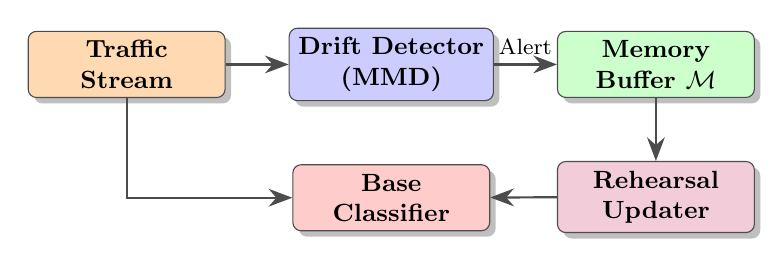
\begin{tikzpicture}[
    node distance=0.9cm and 0.35cm,
    box/.style={rectangle, draw=black!70, fill=#1, minimum width=2.5cm, minimum height=0.8cm, rounded corners=3pt, font=\small\bfseries, align=center, drop shadow},
    arrow/.style={-{Stealth[length=3mm]}, thick, draw=black!70},
    label/.style={font=\footnotesize, align=center}
]
% Main components
\node[box=orange!30] (traffic) {Traffic\\Stream};
\node[box=blue!20, right=0.8cm of traffic] (detector) {Drift Detector\\(MMD)};
\node[box=green!20, right=0.8cm of detector] (buffer) {Memory\\Buffer $\mathcal{M}$};
\node[box=purple!20, below=0.8cm of buffer] (updater) {Rehearsal\\Updater};
\node[box=red!20, below=0.8cm of detector] (classifier) {Base\\Classifier};

% Arrows
\draw[arrow] (traffic) -- (detector);
\draw[arrow] (detector) -- node[above, label] {Alert} (buffer);
\draw[arrow] (buffer) -- (updater);
\draw[arrow] (updater) -- (classifier);
\draw[arrow] (traffic) |- (classifier);
\end{tikzpicture}
\caption{The LightGuard Framework Architecture. The system monitors traffic, detects concept drift using MMD, retrieves historical samples from the managed memory buffer, and performs rehearsal-based model updates to maintain classification accuracy.}
\label{fig:lightguard_architecture}
\end{figure}


\begin{algorithm}[ht!]
\footnotesize
\caption{LightGuard: Continual Learning Update with Adaptive Prioritization}
\label{alg:lightguard_update}
\begin{algorithmic}[1]
\Require Base classifier $f_{\theta}$, Memory buffer $\mathcal{M}$, New data $\mathcal{D}_{new}$, Buffer capacity $M_{max}$, Mini-batch size $B_{\text{size}}$, Prioritization weights $\alpha, \beta, \gamma$
\Ensure Updated classifier $f_{\theta'}$ and memory buffer $\mathcal{M}'$
\Statex
\Function{LightGuardUpdate}{$f_{\theta}, \mathcal{M}, \mathcal{D}_{new}, M_{max}, B_{\text{size}}, \alpha, \beta, \gamma$}
    \State \textbf{Input:} $\mathcal{D}_{new} = \{(x_i, y_i)\}_{i=1}^{N}$ \Comment{New drifted window data}
    \Statex
    \State \textit{\# 1. Construct balanced rehearsal batch (75\% new, 25\% memory)}
    \State $B \gets B_{\text{size}}$ \Comment{e.g., 512}
    \State $B_{\text{new}} \gets \textsc{Sample}(\mathcal{D}_{new}, \lfloor 0.75B \rfloor)$
    \State $B_{\text{mem}} \gets \textsc{Sample}(\mathcal{M}, B - |B_{\text{new}}|)$
    \State $B_{\text{update}} \gets B_{\text{new}} \cup B_{\text{mem}}$
    \Statex
    \State \textit{\# 2. Update model with composite loss (Eq. \ref{eq:rehearsal_loss})}
    \State $\mathcal{L} \gets \frac{1}{|B_{\text{update}}|} \sum_{(x,y) \in B_{\text{update}}} \ell(f_{\theta}(x), y)$
    \State $\theta \gets \theta - \eta \nabla_{\theta} \mathcal{L}$ \Comment{Example: gradient step for differentiable models}
    \State \textbf{or} $f_{\theta} \gets \textsc{Refit}(f_{\theta}, B_{\text{update}})$ \Comment{Example: refit for non-incremental learners (e.g., XGBoost)}
    \Statex
    \State \textit{\# 3. Update memory buffer with adaptive prioritization}
    \State $\mathcal{M} \gets \textsc{PriorityBufferUpdate}(\mathcal{M}, \mathcal{D}_{new}, f_{\theta}, M_{max}, \alpha, \beta, \gamma)$
    \Statex
    \State \Return $f_{\theta}, \mathcal{M}$
\EndFunction
\Statex
\Function{PriorityBufferUpdate}{$\mathcal{M}, \mathcal{D}_{new}, f_{\theta}, M_{max}, \alpha, \beta, \gamma$}
    \State Compute rarity weights $r(y)$ from $\mathcal{D}_{new}$ (normalized inverse class frequency)
    \For{$(x, y) \in \mathcal{D}_{new}$}
        \State $\hat{p} \gets f_{\theta}(x)[y]$ \Comment{Predicted probability for true class $y$}
        \State $p_{\text{total}} \gets \alpha \cdot r(y) + \beta \cdot (1 - \hat{p}) + \gamma \cdot \mathbb{I}(\arg\max f_{\theta}(x) \neq y)$
        \State Add $(x, y, p_{\text{total}})$ to candidate list $C$
    \EndFor
    \State $\mathcal{M}_{\text{all}} \gets \mathcal{M} \cup C$
    \If{$|\mathcal{M}_{\text{all}}| > M_{max}$}
        \State Sort $\mathcal{M}_{\text{all}}$ by $p_{\text{total}}$ (descending) \Comment{Prioritize rare/uncertain/misclassified}
        \State $\mathcal{M} \gets \text{first } M_{max} \text{ samples of } \mathcal{M}_{\text{all}}$
    \Else
        \State $\mathcal{M} \gets \mathcal{M}_{\text{all}}$
    \EndIf
    \State \Return $\mathcal{M}$
\EndFunction
\end{algorithmic}
\end{algorithm}


\subsection{Phase II: The LightGuard Framework Design}
\label{subsec:phase2}

\subsubsection{Architectural Overview}
The core contribution of this work is \emph{LightGuard}, a lightweight continual learning framework designed to autonomously sustain the accuracy of encrypted traffic classifiers under non-stationary network conditions. LightGuard operates as a closed-loop adaptation layer atop an arbitrary base classifier, enabling deployment without architectural modification or full retraining.

The framework is guided by the principle of \emph{informed plasticity}: model updates are triggered only when statistically justified and are executed using a carefully curated balance of new and historical knowledge to prevent catastrophic forgetting. This design explicitly avoids unnecessary retraining and limits computational overhead, making LightGuard suitable for real-world network monitoring systems.

As illustrated in Figure~\ref{fig:lightguard_architecture}, LightGuard consists of three tightly coupled modules that together form an adaptive decision pipeline:

\noindent\textbf{Drift detector.} LightGuard continuously monitors the incoming traffic stream to identify distributional change. Informed by the theoretical foundations in Section~\ref{sec:theoretical_foundations}, it computes the \emph{Maximum Mean Discrepancy (MMD)} between a sliding window of recent traffic features and a reference distribution captured at the last stable model state, providing a quantitative signal of virtual concept drift as formalized in Eq.~\ref{eq:concept_drift}. An update is triggered when the MMD score exceeds a configurable threshold $\tau_{detect}$.

\noindent\textbf{Memory buffer ($\mathcal{M}$).} To mitigate catastrophic forgetting, LightGuard maintains a bounded memory buffer that stores representative samples from prior traffic windows. Unlike naïve FIFO or uniform reservoir sampling, the buffer employs an \emph{adaptive prioritization mechanism} that jointly optimizes two objectives: (1) maintaining approximate class balance to preserve global decision boundaries, and (2) preferentially retaining \emph{rare-class samples} and \emph{hard instances}, such as previously misclassified flows or samples near decision boundaries. By retaining maximally informative historical data, the buffer directly supports the stability--plasticity trade-off formalized in Eq.~\ref{eq:rehearsal_loss}.

\noindent\textbf{Continual learning updater.} Upon a confirmed drift event, the updater executes rehearsal-based adaptation by constructing composite mini-batches that combine newly observed (drifted) samples with prioritized instances from the memory buffer. This balanced sampling injects plasticity through exposure to evolving traffic patterns while reinforcing stability via rehearsal of historical knowledge. The updater then performs a constrained fine-tuning step on the base classifier by minimizing the rehearsal objective in Eq.~\ref{eq:rehearsal_loss}, enabling controlled adaptation without catastrophic forgetting.



 
\begin{figure*}[h!]
    \centering
    \includegraphics[width=1.0\linewidth,height=4.5cm]{\cicaggresults/drift_threshold_ablation_ci.pdf}
    \caption{Drift threshold ablation (mean $\pm$ 95\% CI over 3 seeds). Low thresholds ($\tau\in[0.05,0.10]$) preserve high average F1 by reliably triggering updates, while higher thresholds miss drift events and drive rapid collapse toward the static baseline.}
    \label{fig:drift_threshold}
\end{figure*}


\section{Implementation}
\label{ligh_impl}
\noindent \textit{Base Classifier Selection}: 
The base model \(f_\theta\) in LightGuard is chosen based on Phase I results, selecting the one with the best initial accuracy on \(\mathcal{W}_1\). Due to strong prior performance of tree-based ensembles, LightGuard uses an XGBoost classifier as the primary learner. Because XGBoost does not support true streaming updates (\texttt{partial\_fit}) in the scikit-learn sense, we implement updates by refitting an XGBoost model with the same hyperparameters on the composite update batch (new + replay samples).

\textit{Update Strategy Algorithm}: 
Adaptation follows Algorithm~\ref{alg:lightguard_update}. When drift is detected at time \(t\) (window \(\mathcal{W}_t\)), the updater draws a mini-batch \(B_{new} \sim \mathcal{W}_t\) and a replay batch \(B_{mem} \sim \mathcal{M}\) from memory. These form the training set \(B_{update} = B_{new} \cup B_{mem}\). The base classifier is then updated on \(B_{update}\) via refitting on the composite batch, maintaining stability while reducing the rehearsal objective in Eq.~\ref{eq:rehearsal_loss}. The relative sizes of \(B_{new}\) and \(B_{mem}\) implicitly control \(\lambda\).

\begin{table}[ht!]
\centering
\caption{LightGuard Window-by-Window Performance on the CICDarknet2020 dataset.}
\label{tab:lightguard_windows}
\footnotesize
\setlength{\tabcolsep}{3pt}
\begin{tabular}{ccccc}
\toprule
\textbf{Window} & \textbf{F1} & \textbf{Accuracy} & \textbf{Update} & \textbf{MMD} \\
\midrule
1 & 0.908 & 0.982 & -- & 0.000 \\
2 & 0.940 & 0.964 & \checkmark & 0.108 \\
3 & 0.987 & 1.000 & \checkmark & 0.165 \\
4 & 0.972 & 1.000 & \checkmark & 0.140 \\
5 & 0.959 & 1.000 & \checkmark & 0.118 \\
6 & 0.987 & 1.000 & \checkmark & 0.142 \\
7 & 0.974 & 1.000 & \checkmark & 0.111 \\
8 & 0.972 & 1.000 & \checkmark & 0.141 \\
\midrule
\textbf{Avg} & \textbf{0.962} & \textbf{0.993} & 7 updates & -- \\
\bottomrule
\end{tabular}
\end{table}

\noindent\textit{Sanity check (train/eval separation).}
Several windows in Table~\ref{tab:lightguard_windows} report Accuracy $=1.000$ (values are rounded to three decimals). This does not indicate temporal overlap or train--test contamination: windows are constructed as strictly chronological, non-overlapping time blocks, and each window is evaluated on genuinely future traffic relative to the model state that preceded it. When an update is triggered at window $\mathcal{W}_t$, the update batch is formed only from (i) samples drawn from the current window and (ii) replay samples stored from \emph{prior} windows in the memory buffer. Feature standardization is fit on the initial window and reused thereafter, avoiding any normalization fit on future data. Thus, occasional perfect accuracies reflect separability in specific windows under this protocol (and rounding), not information leakage.

\noindent {\textit{Hyperparameter Configuration}}: LightGuard is configured with a strict memory constraint by setting the buffer size to 5\% of the initial window ($|\mathcal{W}_1|$). The drift detection threshold $\tau_{detect}$ is selected via the drift-threshold sensitivity study reported in Table~\ref{tab:threshold}. During updates, LightGuard uses mini-batches of 512 samples with a 3:1 ratio of new to replay data (75\% from $B_{new}$ and 25\% from $B_{mem}$), operationalizing the stability--plasticity balance.

\subsection{Metrics Definition and Aggregation}
\label{subsec:metrics}
All performance metrics are defined as follows:
Macro-averaged F1-score is the unweighted mean of per-class F1 scores and is our primary metric. Performance decay between windows $i$ and $j$ is computed as an absolute difference, $\Delta = M_i - M_j$, and average decay is the mean of per-window decays relative to the initial window ($\mathcal{W}_1$).
All figures and tables report macro-averaged F1. The “best static model average” refers to the mean F1 across all eight windows for the static XGBoost model.


\begin{figure*}[ht!]
    \centering
    \includegraphics[width=1.0\linewidth,height=11.5cm]{\cicaggresults/visualization_3_lightguard_performance_ci.pdf}
    \caption{Sustained performance of LightGuard vs. static model decay on the CICDarknet2020 dataset (mean $\pm$ 95\% CI over 3 seeds). While the static XGBoost model exhibits monotonic degradation, LightGuard maintains stable, high performance through drift-triggered rehearsal updates.}
    \label{fig:lightguard_performance}
\end{figure*}



\begin{figure*}[ht!]
    \centering
    \includegraphics[width=1.0\linewidth]{\cicresults/visualization_4_tradeoff_analysis.pdf}
    \caption{Efficiency Trade-off Analysis on the CICDarknet2020 dataset. Comparative overhead of three systems: the best static model (Static), LightGuard (LG), and periodic full retraining (Re-Train). LightGuard achieves accuracy comparable to full retraining with a fraction of the computational cost (GPU hours) and minimal memory overhead.}
    \label{fig:tradeoff_analysis}
\end{figure*}

\begin{table}[ht!]
\centering
\caption{Drift Threshold Sensitivity Analysis on the CICDarknet2020 dataset.}
\label{tab:threshold}
\footnotesize
\setlength{\tabcolsep}{2.5pt}
\begin{tabular}{cccc}
\toprule
\textbf{Threshold} & \textbf{Avg F1} & \textbf{Updates} & \textbf{Drift Alerts} \\
\midrule
0.05 & 0.973 & 7.0 & 7.0 \\
0.10 & 0.932 & 6.3 & 6.3 \\
0.15 & 0.572 & 0.6 & 0.6 \\
0.20 & 0.277 & 0.0 & 0.0 \\
0.35 & 0.277 & 0.0 & 0.0 \\
\bottomrule
\end{tabular}
\end{table}


\begin{figure*}[ht!]
    \centering
    \includegraphics[width=1.0\linewidth]{\cicresults/visualization_5_ablation_study.pdf}
    \caption{ Ablation Study \& Buffer Sensitivity. Top: Performance drop when removing core LightGuard components. Bottom: Effect of memory buffer size on average F1-Score on the CICDarknet2020 dataset.}
    \label{fig:ablation_study}
\end{figure*}

\begin{table}[ht!]
\centering
\caption{Ablation Study Results: Impact of Removing Core LightGuard Components.}
\label{tab:ablation}
\footnotesize
\setlength{\tabcolsep}{2.5pt}
\begin{tabular}{lccc}
\toprule
\textbf{Variant} & \textbf{Avg F1} & \textbf{Updates} & \textbf{1-Avg F1} \\
\midrule
Full LightGuard & 0.973 & 7.0 & 0.027 \\
w/o Buffer & 0.505 & 7.0 & 0.495 \\
w/o Detector & 0.681 & 7.0 & 0.319 \\
\bottomrule
\end{tabular}
\end{table}


%\subsubsection{Ablation Study}
To validate the contribution of LightGuard's core components, we conducted an ablation study by systematically disabling them in Section~\ref{abl}. LightGuard w/o Buffer disables the memory buffer $\mathcal{M}$ so that updates use only new data from the drifted window, approximating naive fine-tuning. LightGuard w/o Detector disables drift detection and forces rehearsal-based updates at every window regardless of whether drift is present.



\begin{figure*}[ht!]
    \centering

    % -------- Top image --------
    \subfloat{
        \includegraphics[width=0.95\linewidth]{\cicresults/sota_comparison.pdf}
        \label{fig:sota_top}
    }\\[0.6cm]

    % -------- Bottom image --------
    \subfloat{
        \includegraphics[width=0.95\linewidth]{\vpnresults/sota_comparison.pdf}
        \label{fig:sota_bottom}
    }

    \caption{Comparative performance with continual learning baselines on two datasets: CICDarknet2020 (upper panel) and ISCX-VPN (lower panel). (Left \& Middle) F1-score over time and overall average F1-score for static baselines, LightGuard, and continual learning baselines (Replay Proxy (EWC-style), Replay Proxy (GEM-style), ARF). (Right) Continual learning metrics including Backward Transfer (BWT), Forward Transfer (FWT), and Forgetting.}
    
    \label{fig:sota_comparison}
\end{figure*}





\subsection{Evaluation of LightGuard}

\subsubsection{Durability \& Stability Evaluation}
We evaluated LightGuard on the temporally ordered traffic windows \(\mathcal{W}_1, \ldots, \mathcal{W}_K\) from Phase I. Parameters follow Section \ref{ligh_impl}, with a drift threshold and memory buffer of \(5\%\) of \(|\mathcal{W}_1|\). Figure \ref{fig:lightguard_performance} illustrates LightGuard’s macro-averaged F1-score across windows relative to the static XGBoost baseline. While the static model collapses under drift (final-window macro F1 of 0.088), LightGuard maintains high performance (0.973 average F1 across the horizon in the multi-seed evaluation). Table \ref{tab:lightguard_windows} provides a representative single-seed run with window-wise performance, update triggers, and MMD values (Avg F1 = 0.962), while aggregated plots and tables report mean performance over 3 seeds (Avg F1 = 0.973).

\subsubsection{Efficiency \& Operational Overhead Analysis}
Operational viability depends on efficiency. We logged inference latency per flow, update duration, and total memory usage (model + buffer). Figure \ref{fig:tradeoff_analysis} compares three systems: static XGBoost (Static), LightGuard (LG), and periodic full retraining (Re-Train). LightGuard achieves performance comparable to periodic retraining while requiring substantially fewer update operations and a small, fixed memory budget (5\% buffer). The static model, while lightweight, suffers severe performance decay.




\begin{table*}[ht!]
\centering
\caption{Performance Comparison with State-of-the-Art Continual Learning Methods on Two Encrypted Traffic Datasets. Results are reported in terms of Average F1-Score, Final F1-Score, Backward Transfer (BWT), and Forgetting for CICDarknet2020 and ISCX-VPN.}
\label{tab:sota_comparison}
\setlength{\tabcolsep}{2.5pt}
\begin{tabular}{lcccccccc}
\toprule
& \multicolumn{4}{c}{\textbf{CICDarknet2020 (XGBoost)}} & \multicolumn{4}{c}{\textbf{ISCX-VPN (XGBoost)}} \\
\cmidrule(lr){2-5} \cmidrule(lr){6-9}
\textbf{Method} 
& \textbf{Avg F1} & \textbf{Final F1} & \textbf{BWT} & \textbf{Forgetting}
& \textbf{Avg F1} & \textbf{Final F1} & \textbf{BWT} & \textbf{Forgetting} \\
\midrule

Static XGB
&0.297 &0.088 &-0.781 &0.894
&0.503 &0.527 &-0.490 &0.405 \\

ARF
&0.507 &0.475 &0.060 &0.295
&0.205 &0.259 &0.015 &0.034 \\

Replay Proxy (EWC-style)
&0.729 &0.660 &-0.237 &0.276
&0.626 &0.675 &-0.285 &0.200 \\

Replay Proxy (GEM-style)
&0.729 &0.660 &-0.237 &0.276
&0.626 &0.675 &-0.285 &0.200 \\

\textbf{LightGuard}
& \textbf{0.973} & \textbf{0.999} & \textbf{0.061} & \textbf{0.001}
& \textbf{0.796} & \textbf{0.896} & \textbf{-0.098} & \textbf{0.027} \\
\bottomrule
\end{tabular}

\caption*{\footnotesize
\textit{Note:} LightGuard uses XGBoost as the base learner. All methods are evaluated over eight temporal windows under an identical windowing protocol; CICDarknet2020 results are aggregated over 3 seeds, while ISCX-VPN results are reported from a single run.
}
\end{table*}



\subsection{Ablation \& Sensitivity Studies}
\label{abl}

We evaluated LightGuard's sensitivity to key hyperparameters. The drift detection threshold $\tau_{detect}$ is critical: when $\tau \geq 0.15$, missed drift events substantially reduce adaptation frequency and degrade performance, and by $\tau \geq 0.20$ the system effectively reverts to the static baseline. In contrast, low thresholds ($\tau\in[0.05,0.10]$) sustain high average F1 by reliably triggering updates. In the multi-seed study, $\tau=0.05$ maximizes average macro F1 (0.973) but triggers updates in essentially every post-training window, while $\tau=0.10$ reduces the update rate (6.32 updates on average over 7 opportunities) at a modest cost in average macro F1 (0.932). Unless otherwise stated, comparative results use $\tau=0.05$ to report the best-performing operating point under this evaluation.

Ablation studies (Table \ref{tab:ablation}, Figure \ref{fig:ablation_study}) show that both the memory buffer and drift detector are essential. Without the buffer, average F1 drops to 0.505, consistent with catastrophic forgetting under naive fine-tuning. Without drift detection, average F1 drops to 0.681, reflecting the cost of frequent, non-selective updates. Together, these results indicate that durability requires both (i) rehearsal to preserve historical decision regions and (ii) event-driven updates to avoid unnecessary retraining.

In Figure \ref{fig:ablation_study} (right panel), we also analyzed memory buffer size $\mathcal{M}$ as a fraction of $|\mathcal{W}_1|$. Performance improves sharply when moving from very small buffers to moderate buffers, and then saturates, indicating diminishing returns beyond a small memory footprint. We adopt 5\% as a practical operating point.


 
\subsection{Comparison with Continual Learning Baselines}
\label{subsec:sota_comparison}
We compare LightGuard against baselines that are compatible with the windowed evaluation protocol: a static XGBoost model (no updates), Adaptive Random Forest (ARF), and two replay-style proxy baselines that refit the base learner on a small class-balanced memory buffer plus a small sample from the current window. We denote these as \emph{Replay Proxy (EWC-style)} and \emph{Replay Proxy (GEM-style)} to reflect their inspiration while making clear they are pragmatic replay baselines in a tree-ensemble setting, not faithful implementations of the original gradient-based neural methods.

All methods are evaluated using: (1) \textit{Average F1-Score} across windows; (2) \textit{Final F1-Score} on the last window; (3) \textit{Backward Transfer (BWT)}; (4) \textit{Forward Transfer (FWT)}; and (5) \textit{Forgetting}. All methods share identical features, windows, and random seeds. Table~\ref{tab:sota_comparison} summarizes results on CICDarknet2020 and ISCX-VPN; LightGuard consistently outperforms the static baseline and reduces forgetting.

\subsection{Discussion of Findings} 
LightGuard successfully addresses \textit{durability deception}, maintaining an average F1-score of 0.973 on CICDarknet2020 with a 5\% memory buffer. In contrast, the static XGBoost baseline achieves only 0.297 average F1 and collapses to 0.088 macro F1 in the final window. These results indicate that durability under drift is attainable with lightweight, event-driven continual learning rather than periodic full retraining.

Key findings: (1) Performance advantage is consistent across CICDarknet2020 and ISCX-VPN, showing generalizability. (2) LightGuard outperforms replay-style proxy baselines and ARF under the same windowed protocol (Table~\ref{tab:sota_comparison}), confirming that gains stem from the adaptation strategy. (3) LightGuard requires fewer updates than periodic retraining, showing drift-aware efficiency.

From a security operations perspective, LightGuard converts encrypted-traffic classifiers from disposable tools into long-term assets, reducing post-deployment maintenance burden and durability risk. This enables real-time monitoring without excessive cost, making durable visibility into privacy-channel usage feasible.

\noindent \textit{\textbf{Limitation:}} This study's primary limitation is its reliance on laboratory datasets to simulate drift. While both CICDarknet2020 and ISCX-VPN provide valid testbeds, future work must validate LightGuard on real, continuous streams of timestamped network traffic from production environments. Furthermore, our current framework assumes a fixed set of traffic classes and immediate label availability. A critical avenue for future research is extending LightGuard to handle \textit{open-set recognition}, where entirely new, unseen traffic categories emerge, and to operate under delayed and noisy supervision. Addressing these challenges will further bridge the gap between laboratory research and operational deployment of resilient ML-based security systems.

 
\section{Conclusion}
\label{sec:conclusion}
This study identifies and quantifies the \textit{durability deception} phenomenon in encrypted traffic classification, showing via longitudinal analysis on CICDarknet2020 that static models can suffer severe performance collapse under temporal concept drift. Under chronological evaluation, a static XGBoost classifier degrades from 0.983 macro F1 in Window~1 to 0.088 in Window~8, with accuracy dropping from 0.997 to 0.213, demonstrating that strong in-distribution performance is not a reliable proxy for post-deployment durability. To address this failure mode, we propose \textit{LightGuard}, a lightweight continual learning framework that couples statistically grounded drift detection with stability-preserving rehearsal. On CICDarknet2020, LightGuard sustains 0.973 average macro F1 across the horizon with only a 5\% memory buffer, substantially reducing forgetting while maintaining operational efficiency. Validation on ISCX-VPN supports the generalizability of these findings. Overall, this work shifts evaluation from one-time accuracy to long-horizon resilience and provides a practical pathway toward sustainable, drift-aware encrypted traffic monitoring. Future work will relax the idealized label-availability assumption and validate LightGuard on continuous production streams with delayed and noisy supervision.
 
\appendices
\section{Additional Dataset Availability (Appendix)}
\label{app:ids2018}
In addition to CICDarknet2020 and ISCX-VPN, we document a large-scale intrusion dataset, CSE-CIC-IDS2018, for reproducibility and future extension of our evaluation suite. The dataset is officially distributed as a public AWS S3 bucket (not a single CSV URL) and can be obtained without an AWS account using the AWS CLI:\\
\texttt{aws s3 sync --no-sign-request --region ca-central-1 "s3://cse-cic-ids2018/" <dest-dir>}.\\
For details, see the AWS Open Data Registry entry~\cite{cse_cic_ids2018}.

\bibliographystyle{IEEEtran}
 \bibliography{references}

\end{document}


